
\newcommand{\pol}{\ensuremath{\pi}}
\newcommand{\optpol}{\ensuremath{{\pol}_\ast}}
\newcommand{\polset}{\ensuremath{\Pi}}
%\newcommand{\curs}{{s_\mathrm{C}}}
\newcommand{\curs}{s}
\newcommand{\cura}{a}
%\newcommand{\nexta}{{a_{N}}}
%\newcommand{\nexts}{{s_{N}}}
\newcommand{\nexta}{{a'}}
\newcommand{\nexts}{{s'}}
\newcommand{\condsetbig}[2]{\left\{\left.#1\right|#2\right\}}
\newcommand{\condprobbig}[2]{p\left(\left.#1\right|#2\right)}
\newcommand{\Condprobbig}[2]{P\left(\left.#1\right|#2\right)}
\newcommand{\df}{\ensuremath{\gamma}}
\newcommand{\condprobb}[2]{p(#1|#2)}
\newcommand{\suppk}[1]{\ensuremath{\mathcal{#1}}}
\newcommand{\suppx}{\suppk{X}}
\newcommand{\suppy}{\suppk{Y}}
\newcommand{\suppz}{\suppk{Z}}
\renewcommand{\Expect}{\mathbf{E}}

\newcommand{\stateset}{\ensuremath{\mathcal{S}}}
\newcommand{\nonterminalstateset}{{\stateset'}}
\newcommand{\actionset}{\ensuremath{\mathcal{A}}}
\newcommand{\numstates}{{|\stateset|}}

\newcommand{\assign}{\leftarrow}
\newcommand{\epsgreedy}{$\epsilon$-greedy}
\newcommand{\epssoft}{$\epsilon$-soft}
\newcommand{\reward}[1]{\ensuremath{R_{#1}}}
\newcommand{\return}[1]{\ensuremath{G_{{#1}}}}
\newcommand{\state}[1]{\ensuremath{S_{#1}}}
\newcommand{\action}[1]{\ensuremath{A_{#1}}}
\newcommand{\nstepreturn}[2]{G_{{#1}:{#2}}}
\newcommand{\nstepqreturn}[2]{G^{Q}_{{#1}:{#2}}}
\newcommand{\tdparam}{\ensuremath{\lambda}}
\newcommand{\ldreturn}[1]{G^{\tdparam}_{#1}}
\newcommand{\stepsize}[1]{\ensuremath{\alpha_{#1}}}
\newcommand{\tderror}[1]{\ensuremath{\delta_{#1}}}
\newcommand{\tderrorvar}[1]{\ensuremath{\delta'_{#1}}}

\newcommand{\et}[1]{\ensuremath{z_{#1}}}
\newcommand{\wvector}[1]{\ensuremath{{w_{#1}}}}

\newcommand{\defeq}{\coloneqq}

\newcommand{\valappr}{\ensuremath{\hat{v}}}

\newcommand{\wvectdim}{d}

\newcommand{\indexstatemapping}{\ensuremath{\phi}}




%\def\beginalg#1\endalg{%
%\begin{center}\framebox{\vbox{\begin{tabbing}%
%#1%
%\end{tabbing}}}\end{center}%
%}

\newcommand{\alggap}{0.7cm}

\def\beginalg#1\endalg{%
\begin{center}\framebox{\vbox{\begin{tabbing}%
\hspace*{\alggap}\=\hspace*{\alggap}\=\hspace*{\alggap}\=\hspace*{\alggap}\=%
\hspace*{\alggap}\=\hspace*{\alggap}\=\hspace*{\alggap}\=\hspace*{\alggap}\= \kill%
#1%
\end{tabbing}}}\end{center}%
}

\def\balg#1\ealg{
\begin{center}%
\frame{%
\begin{varwidth}{\linewidth}%
\begin{tabbing}%
#1%
\end{tabbing}%
\end{varwidth}%
}%
\end{center}%
}

The reinforcement learning is a machine learning where an agent learns how to take actions to achieve a goal
by maximizing cumulative reward while interacting with environment.
Learning from interaction is a foundational idea underlying nearly all theories of learning and intelligence.

It differs from supervised learning in that labeled input and output pairs need not be presented
(and sub-optimal actions need not be explicitly corrected).
Instead the focus is finding a balance between exploration of uncharted territory and exploitation of current knowledge.
It is much more focused on goal-directed learning from interaction than other approaches to machine learning.

In the following sections,
we introduce finite Markov decision process (MDP)
and three typical methods to solve reinforcement learning problems.
All these methods are called tabular solution methods
because they need to store values for all the states or all the state-action pairs (that have been visited).

%Here we primarily explore idealized learning situations and evaluate the effectiveness of various learning methods.


\section{Finite Markov decision processes}

We introduce the formal problem of finite Markov decision processes (MDPs),
which we try to solve.
This problem involves evaluative feedback,
but also an associative aspect, \ie, choosing different actions in different situations.
MDP is a classical formalization of sequential decision making,
where actions influence not just immediate rewards,
but also subsequent states through those future rewards.
Thus MDPs involve delayed reward and the need to trade-off immediate and delayed reward.

\figurename~\ref{fig:mdp} depicts MDP where an agent interacts with environment.
The current state of the environment is known to the agent.
With knowledge of state, the agent makes a decision as to which action to take.
This action, in turn, will change the state of the environment and the agent will receive
a reward at the same time.
The agent remembers this reward in some indirect way and uses it for making future decisions.

\begin{figure}
\begin{center}
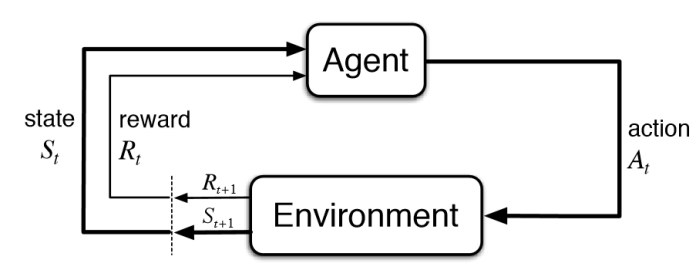
\includegraphics[width=.7\textwidth]{figures/reinforcement-learning}
\end{center}
\caption{The agent-environment interaction in a Markov decision process.}
\label{fig:mdp}
\end{figure}


\subsection{Markov property}


Suppose that the agent is in state \state{t}\ takes action \action{t}\ at time $t$.
Then the agent receives reward \reward{t+1}\ (from the environment) and the environment transitions to state \state{t+1}.
MDP assumes that all these quantities are random variables.

Let \stateset\ and \actionset\ be the set of all the states and that of all the actions the agent can take respectively.

Now suppose that the environment is in state $\state{0}\in\stateset$ the agent takes action $\action{0}\in\actionset$ at $t=0$.
Then the state of the environment becomes $\state{1}\in\stateset$ giving the agent $\reward{1}\in\reals$ as reward.
Suppose that the agent repeat taking actions.

Then we have a sequence of random variables
\begin{equation}
\state{0}, \action{0},
\reward{1}, \state{1}, \action{1},
\reward{2}, \state{2}, \action{2},
\reward{3}, \state{3}, \action{3},
\ldots
\end{equation}

We assume that these random variables satisfy the Markov Property (as assumed by the name) in the following sense.

\begin{equation}
\state{t+1}, \reward{t+1} | \state{t}, \action{t}, \reward{t}, \state{t-1}, \action{t-1}, \reward{t-1}, \ldots
= \state{t+1}, \reward{t+1} | \state{t}, \action{t}
\end{equation}
\ie, two random variables, \state{t+1}\ and \reward{t+1}, conditioned on every state, action, and reward before $t+1$
are the same as those conditioned on \state{t}\ and \reward{t}\ only.

This can be formally expressed using the probability density function (PDF)
as follows.
\begin{equation}
\condprobbig{\state{t+1}, \reward{t+1} }{ \state{t}, \action{t}, \reward{t}, \state{t-1}, \action{t-1}, \reward{t-1}, \ldots}
= \condprobbig{\state{t+1}, \reward{t+1} }{ \state{t}, \action{t} }.
\end{equation}

This is the reason that the process is called \emph{Markov} decision process.

\subsection{Policy}

The \emph{policy} is defined by the conditional probability of \action{t}\ given \state{t},
\ie,
\begin{equation}
\pol(A|S) = \condprobb{A_t}{\state{t}},
\end{equation}
which implies the probability of taking certain action depends only on the current state, not the time.
The policy decides which actions the agent takes in each state.

Let \polset\ be the set of all the policies.

\subsection{Return}

The \emph{return} at $t$ is defined by
\begin{equation}
        G_t
        = \sum_{k=0}^\infty \gamma^k \reward{t+k}
        = \reward{t+1} + \gamma \reward{t+2} + \gamma^2 \reward{t+3} + \cdots
\end{equation}
where $\gamma \in [0,1]$ is called the \emph{discount factor}.
If $\gamma=0$, the agent is myopic, \ie, it only cares the immediate reward.
If $\gamma=1$, the agent is truly far-sighted, \ie, it cares all the future rewards without discounting.
If $\gamma$ is somewhere between $0$ and $1$, it considers near-future rewards more importantly than those in far future.


\subsection{State value function and action value function}

The state value function (which is sometimes referred to as just value function) is defined by
\begin{equation}
v_\pol(\curs)
= \Expect_{\pol,p} \condsetbig{G_{t}}{\state{t} = \curs}
= \Expect_{\pol,p} \condsetbig{
    \sum_{k=0}^\infty \gamma^k \reward{t+k}
    }{\state{t} = \curs}.
\end{equation}
In other words, the state value function is a function of a state
representing the expected return the agent will get from the state
when following the policy $\pol$.

The action value function (which is sometimes referred to as just action function) is defined by
\begin{equation}
q_\pol(\curs, \cura)
= \Expect_{\pol,p} \condsetbig{G_{t}}{\state{t} = \curs, A_t = \cura}
= \Expect_{\pol,p} \condsetbig{
    \sum_{k=0}^\infty \gamma^k \reward{t+k}
    }{\state{t} = \curs, A_t = \cura}.
\end{equation}
In other words, the action value function is a function of a state and an action
representing the expected return the agent will get from the state when the agent takes a certain action
and follows the policy $\pol$.

As mentioned above, most reinforcement learning algorithms try to maximize either one of these functions,
\ie,
not maximizing the immediate reward, but the long-term return.

%\newpage
\section{Bellman equation}

\href{https://en.wikipedia.org/wiki/Richard_E._Bellman}{Richard E. Bellman}, who introduced dynamic programming in $1953$,
proposed an equation as a necessary condition for optimality associated with dynamic programming,
which is called Bellman equation.
One of the properties that Markov property implies is that the value functions only depend on the current state (and the action taken)
and that the function value is closely related to the function values of the next states.
These facts are cleverly used to derive the Bellman equation.
Here we introduce two Bellman equations; one for the state value function and the other for action value function.


\subsection{Bellman equations}

To derive Bellman equations, we use some basic statistics facts regarding conditional expectations.
(Refer to \S\ref{sec:rl-app}.)

Since the definitions of state value function and action value function together with (\ref{eq:dkci}) imply
\begin{eqnarray*}
v_\pol(\curs)
&=& \Expect_{\pol,p} \condsetbig{G_{t}}{\state{t} = \curs}
\\
&=& \Expect_{A_t|\state{t} =\curs} \Expect_{\pol,p} \condsetbig{G_{t}}{\state{t} = \curs, A_t}
\\
&=& \sum_\cura p(A_t=\cura|\state{t} =\curs) \Expect_{\pol,p} \condsetbig{G_{t}}{\state{t} = \curs, A_t=\cura}
\\
&=& \sum_\cura \pol(\cura|\curs) \Expect_{\pol,p} \condsetbig{G_{t}}{\state{t} = \curs, A_t=\cura}
\\
&=& \sum_\cura \pol(\cura|\curs) q_\pol(\curs,\cura)
\end{eqnarray*}
and
\begin{eqnarray*}
q_\pol(\curs, \cura)
&=& \Expect_{\pol,p} \condsetbig{G_{t}}{\state{t} = \curs, A_t = \cura}
\\
&=& \Expect_{\state{t+1}, \reward{t+1}|\state{t}=\curs,A_t=\cura} \Expect_{\pol,p} \condsetbig{G_{t}}{\state{t} = \curs, A_t = \cura, \state{t+1}, \reward{t+1} }
\\
&=& \Expect_{\state{t+1}, \reward{t+1}|\state{t}=\curs,A_t=\cura} \Expect_{\pol,p} \condsetbig{\sum_{k=0}^\infty \df^k \reward{t+k+1}}{\state{t} = \curs, A_t = \cura, \state{t+1}, \reward{t+1} }
\\
&=& \Expect_{\state{t+1}, \reward{t+1}|\state{t}=\curs,A_t=\cura} \Expect_{\pol,p} \condsetbig{\reward{t+1} + \df \sum_{k=0}^\infty \df^k \reward{t+k+2}}{\state{t} = \curs, A_t = \cura, \state{t+1}, \reward{t+1} }
\\
&=& \sum_{\nexts, r} p_{\state{t+1}, \reward{t+1}|\state{t},A_t}(\nexts, r|\curs,\cura) \Expect_{\pol,p} \condsetbig{\reward{t+1} + \df G_{t+1} }{\state{t} = \curs, A_t = \cura, \state{t+1} = \nexts, \reward{t+1} =r}
\\
&=& \sum_{\nexts, r} p_{\state{t+1}, \reward{t+1}|\state{t},A_t}(\nexts, r|\curs,\cura) \left( r + \df \Expect_{\pol,p} \condsetbig{G_{t+1}}{\state{t} = \curs, A_t = \cura, \state{t+1} = \nexts, \reward{t+1} =r} \right)
\\
&=& \sum_{\nexts, r} p_{\state{t+1}, \reward{t+1}|\state{t},A_t}(\nexts, r|\curs,\cura) \left( r + \df \Expect_{\pol,p} \condsetbig{G_{t+1}}{\state{t+1} = \nexts} \right)
\\
&=& \sum_{\nexts, r} p_{\state{t+1}, \reward{t+1}|\state{t},A_t}(\nexts, r|\curs,\cura) \left( r + \df v_\pol(\nexts) \right),
\end{eqnarray*}
we have the following two equations relating state value function to action value function and vise versa.
\begin{equation}
\label{eq:rel:v-a}
v_\pol(\curs) = \sum_\cura \pol(\cura|\curs) q_\pol(\curs,\cura).
\end{equation}
\begin{equation}
\label{eq:rel:a-v}
q_\pol(\curs, \cura)
= \sum_{\nexts, r} p_{\state{t+1}, \reward{t+1}|\state{t},A_t}(\nexts, r|\curs,\cura) \left( r + \df v_\pol(\nexts) \right).
\end{equation}

Now (\ref{eq:rel:v-a}) and (\ref{eq:rel:a-v}) imply that
\begin{equation}
\label{eq:bellman:state}
v_\pol(\curs)
= \sum_\cura \pol(\cura|\curs) q_\pol(\curs,\cura)
= \sum_\cura \pol(\cura|\curs) \sum_{\nexts, r} p(\nexts, r|\curs,\cura) \left( r + \df v_\pol(\nexts) \right)
\end{equation}
and
\begin{equation}
\label{eq:bellman:action}
q_\pol(\curs,\cura)
= \sum_{\nexts, r} p(\nexts, r|\curs,\cura) \left( r + \df v_\pol(\nexts) \right)
= \sum_{\nexts, r} p(\nexts, r|\curs,\cura) \left( r + \df \sum_\nexta \pol(\nexta|\nexts) q_\pol(\nexts,\nexta) \right).
\end{equation}

The equation (\ref{eq:bellman:state}) is called \emph{Bellman equation for state value function}
and the equation (\ref{eq:bellman:action}) is called \emph{Bellman equation for action value function}.

\subsection{Bellman optimality equations}

Now suppose that the policy \optpol\ is the optimal policy.
Then we define the \emph{optimal state-value function}
as that of \optpol, \ie,
\begin{equation}
v_\ast(\curs) = v_{\optpol}(\curs) = \max_{\pol\in\polset} v_\pol(\curs).
\end{equation}
Likewise,
we define the \emph{optimal action-value function}
as that of \optpol, \ie,
\begin{equation}
q_\ast(\curs,\cura) = q_{\optpol}(\curs,\cura) = \max_{\pol\in\polset} q_\pol(\curs,\cura).
\end{equation}

Then (\ref{eq:rel:v-a}) and (\ref{eq:rel:a-v}) imply that
\begin{equation}
\label{eq:bellman:opt:state}
v_\ast(\curs) = v_{\optpol}(\cura) = \max_{\cura\in\actionset} q_{\optpol}(\curs,\cura)
= \max_{\cura\in\actionset} \sum_{\nexts, r} p(\nexts, r|\curs,\cura) \left( r + \df v_\pol(\nexts) \right).
\end{equation}
and
\begin{equation}
\label{eq:bellman:opt:action}
q_\ast(\curs,\cura)
= q_{\optpol}(\curs,\cura)
= \sum_{\nexts, r} p(\nexts, r|\curs,\cura) \left( r + \df v_{\optpol}(\nexts) \right).
= \sum_{\nexts, r} p(\nexts, r|\curs,\cura) \left( r + \df \max_{\nexta\in\actionset}q_{\optpol}(\nexts, \nexta) \right).
\end{equation}

The equation (\ref{eq:bellman:opt:state}) is called \emph{Bellman optimality equation for state value function}
and the equation (\ref{eq:bellman:opt:action}) is called \emph{Bellman optimality equation for action value function}.


%\newpage
\section{Dynamic programming}

The term dynamic programming (DP)
refers to a collection of algorithms that
can be used to compute optimal policies given a perfect model of the environment as a Markov decision process (MDP).
DP provides an essential foundation for the understanding of the methods presented in the rest of this chapter.
All of these methods can be viewed as attempts to achieve much the same effect as DP,
only with less computation and without assuming a perfect model of the environment.

The key idea of DP, and of reinforcement learning generally, is the use of value functions to organize and structure the search for good policies.


\subsection{Policy evaluation (prediction)}

We consider how to compute the state-value function $v_\pol$ for an arbitrary policy \pol.
This is called \emph{policy evaluation} in the DP literature. We also refer to it as the \emph{prediction problem}.
The existence and uniqueness of $v_\pol$ are guaranteed as long as either $\df < 1$
or eventual termination is guaranteed from all states under the policy $\pol$.

The policy evaluation algorithm uses the fact that all the state value functions satisfy the Bellman equation for state value function.
We use this equation, but in an iterative manner.
\begin{equation}
v_{k+1}(\curs)
\assign \sum_\cura \pol(\cura|\curs) \sum_{\nexts, r} p(\nexts, r|\curs,\cura) \left( r + \df v_{k}(\nexts) \right).
\end{equation}
This equation resembles (\ref{eq:bellman:state}), but different because now we put subscript $k$ in place of the policy \pol.
Indeed, the sequence $v_k$
can be shown in general to converge to $v_\pol$ as $k$ goes to $\infty$
the same conditions that guarantee the existence of $v_\pol$.
This algorithm is called \emph{iterative policy evaluation}.

We can consider \emph{in-place} version of this algorithm,
\ie, we replace the values for $v_k$ for each state without waiting until we sweep all the states for one iteration.
This in-place algorithm also converges to $v_\pol$.
In fact, it usually converges faster.
This in-place algorithm is described in \tablename~\ref{tab:alg:policy-evaluation}.


\begin{table}
\beginalg
Inputs: \pol, MDP \\
Algorithm parameters: $\theta > 0$ (small threshold determining accuracy of estimation)\\
\\
Initialize $V(\curs) \in \reals$ for all $\curs \in \stateset$ except that $V(\mathrm{terminal}) = 0$ \\
\\
 Loop: \\
 \> $\Delta \assign 0$ \\
 \> For each $s\in\stateset$: \\
 \> \> $v\assign V(\curs)$ \\
 \> \> $V(s) \assign \sum_\cura \pol(\cura|\curs) \sum_{\nexts, r} p(\nexts, r|\curs,\cura) \left( r + \df V(\nexts) \right)$ \\
 \> \> $\Delta \assign \max\{\Delta, |v-V(s)|\}$ \\
 until $\Delta < \theta$
\endalg
\caption{Iterative Policy Evaluation for estimating $V \sim v_\pol$}
\label{tab:alg:policy-evaluation}
\end{table}


\subsection{Policy iteration}

The policy iteration is the iterative process of improving policy as to maximize the value functions.
The algorithm is described in \tablename~\ref{tab:eq:policy-iteration}.

\begin{table}
\beginalg
Inputs: MDP \\
Algorithm parameters: $\theta > 0$ (small threshold determining accuracy of estimation)\\
\\
1. Initialization \\
\> $V(\curs) \in \reals$ and $\pol(s) \in \actionset(s)$ for all $s\in\stateset$\\
\\
2. Policy Evaluation\\
\> Loop: \\
\> \> $\Delta \assign 0$ \\
\> \> For each $s\in\stateset$: \\
\> \> \> $v\assign V(\curs)$ \\
\> \> \> $V(s) \assign \sum_\cura \pol(\cura|\curs) \sum_{\nexts, r} p(\nexts, r|\curs,\cura) \left( r + \df V(\nexts) \right)$ \\
\> \> \> $\Delta \assign \max\{\Delta, |v-V(s)|\}$ \\
\> until $\Delta < \theta$\\
\\
3. Policy Improvement\\
$u \assign {\tt true}$\\
\> For each $\curs \in \stateset$\\
\> \> $b \assign \pol(\curs)$\\
\> \> $\pol(\curs) \assign \sum_\cura \pol(\cura|\curs) \sum_{\nexts, r} p(\nexts, r|\curs,\cura) \left( r + \df v_\pol(\nexts) \right)$\\
\> \> If $b \neq \pol(\curs)$, then $t \assign {\tt false}$\\
\> If $u$, then stop and return $V \sim v_\ast$ and $\pol \sim \optpol$; else go to 2
\endalg
\caption{Policy Iteration (using iterative policy evaluation) for estimating $\pol \sim \optpol$.}
\label{tab:eq:policy-iteration}
\end{table}


\subsection{Value iteration}

One drawback to policy iteration is that each of its iterations involves policy evaluation.
In fact, the policy evaluation step of policy iteration can be truncated in several ways
without losing the convergence guarantees of policy iteration.
One important special case is when policy evaluation is stopped after just one sweep (one update of each state).
This algorithm is called \emph{value iteration}.
It can be written as a particularly simple update operation that combines the policy improvement and truncated policy evaluation steps.
\begin{equation}
v_{k+1}(\curs) \assign \max_{\cura\in\actionset} \sum_{\nexts, r} p(\nexts, r|\curs,\cura) \left( r + \df v_k(\nexts) \right).
\end{equation}
Note that value iteration is obtained simply by turning the Bellman optimality equation for state value function
(\ref{eq:bellman:opt:state})
into an update rule.

The in-place version of value iteration algorithm is described in \tablename~\ref{tab:alg:value-iteration}.

\begin{table}
\beginalg
Inputs: MDP \\
Algorithm parameters: $\theta > 0$ (small threshold determining accuracy of estimation)\\
\\
Initialize $V(\curs) \in \reals$ for all $\curs \in \stateset$ except that $V(\mathrm{terminal}) = 0$ \\
\\
Loop: \\
\> $\Delta \assign 0$ \\
\> For each $s\in\stateset$: \\
\> \> $v\assign V(\curs)$ \\
\> \> $V(s) \assign \max_{\cura\in\actionset(\curs)} \sum_{\nexts, r} p(\nexts, r|\curs,\cura) \left( r + \df V(\nexts) \right)$ \\
\> \> $\Delta \assign \max\{\Delta, |v-V(s)|\}$ \\
until $\Delta < \theta$\\
\\
Output: deterministic policy $\pol$ such that\\
\> $\pol(\curs) = \argmax_{\cura\in\actionset(\curs)} \sum_{\nexts, r} p(\nexts, r|\curs,\cura) \left( r + \df V(\nexts) \right)$
\endalg
\caption{Value Iteration for estimating $\pol \sim \optpol$}
\label{tab:alg:value-iteration}
\end{table}



%\newpage
\section{Monte Carlo methods}

Here we consider learning methods for estimating value functions and discovering optimal policies.
Unlike the previous methods,
we do not assume complete knowledge of the environment.
Monte Carlo (MC) methods require only experience sample sequences of states, actions, and rewards
from \emph{actual or simulated interaction with an environment}.
Learning from actual experience is striking because it requires no prior knowledge of the environment’s dynamics,
yet can still attain optimal behavior.
\emph{Learning from simulated experience is also powerful.}
Although a model is required,
the model need only generate sample transitions,
\emph{not the complete probability distributions of all possible transitions} that is required for dynamic programming (DP).

MC methods are ways of solving the reinforcement learning problem based on averaging sample returns.
To ensure that well-defined returns are available, here we define Monte Carlo methods only for episodic tasks.

Monte Carlo methods sample and average returns for each state–action pair much like the bandit methods
where we sample and average rewards for each action.
The main difference is that now there are multiple states,
each acting like a different bandit problem (like an associative-search or contextual bandit)
and the different bandit problems are interrelated.
That is, the return after taking an action in one state depends on the actions taken in later states in the same episode.
Because all the action selections are undergoing learning, the problem becomes nonstationary from the point of view of the earlier state.


To handle the nonstationarity,
we adapt the idea of general policy iteration (GPI) developed for DP.
Whereas there we computed value functions from knowledge of the MDP,
here we learn value functions from sample returns with the MDP.
The value functions and corresponding policies still interact to attain optimality
in essentially the same way (GPI).
As in DP,
first we consider the prediction problem, then policy improvement, and, finally,
the control problem and its solution by GPI.
Each of these ideas taken from DP is extended to the Monte Carlo case in which only sample experience is available.


\subsection{Monte Carlo prediction}

An obvious way to estimate it from experience, then, is simply to average the returns observed after visits to that state.
There are two Monte Carlo (MC) prediction methods; \emph{first-visit MC method} and \emph{every-visit MC method}.
These two MC methods are very similar but have slightly different theoretical properties.
First-visit MC has been most widely studied, dating back to the 1940s.
Every-visit MC extends more naturally to function approximation and eligibility traces.

\tablename~\ref{tab:alg:first-visti-mc-prediction} describes the first-visit MC prediction algorithm.


\begin{table}
\beginalg
Inputs: \pol\\
\\
Initialize:\\
\> $V(\curs) \in \reals$ for all $\curs\in\stateset$\\
\> $R(\curs) \assign {\tt list()}$ for all $\curs\in\stateset$\\
\\
Loop: \\
\> Generate an episode following \pol: $\state{0}, \action{0}, \reward{1}, \state{1}, \action{1}, \reward{2}, \ldots, \state{T-1}, \action{T-1}, \reward{T}$\\
\> $G \assign 0$\\
\> Loop for each step of episode, $t+T-1, T-2, \ldots, 0$:\\
\> \> $G \assign \df G + \reward{t+1}$\\
\> \> If $\state{t} \not\in \{\state{0}, \state{1}, \ldots, \state{t-1}\}$:\\
\> \> \> $R(\state{t}){\tt.append}(G)$\\
\> \> \> $V(\state{t}) \assign R(\state{t}){\tt .average()}$\\
Until a certain criterion is satisfied
\endalg
\caption{First-visit MC prediction for estimating $V \sim v_\pol$}
\label{tab:alg:first-visti-mc-prediction}
\end{table}


\subsection{Monte Carlo control}

The overall idea is to proceed according to the same pattern as in the dynamic programming, \ie,
according to the idea of generalized policy iteration (GPI).
In GPI one maintains both an approximate policy and an approximate value function.
The value function is repeatedly altered to more closely approximate
the value function for the current policy,
and the policy is repeatedly improved with respect to the current value function.
These two kinds of changes work against each other to some extent,
as each creates a moving target for the other,
but together they cause both policy and value function to approach optimality.

For Monte Carlo policy evaluation
it is natural to alternate between evaluation and improvement on an episode-by-episode basis.
After each episode,
the observed returns are used for policy evaluation,
and then the policy is improved at all the states visited in the episode.
A complete simple algorithm along these lines, which is called Monte Carlo ES for Monte Carlo with Exploring Starts,
is described in \tablename~\ref{tab:alg:mc-es-control}.


\begin{table}
\beginalg
Initialize:\\
\> $\pol(\curs) \in \actionset(\curs)$ for all $\curs\in\stateset$\\
\> $Q(\curs,\cura) \in \reals$ for all $\curs\in\stateset$ and $\cura\in\actionset(\curs)$\\
\> $R(\curs, \cura) \assign {\tt list()}$ for all $\curs\in\stateset$ and $\cura\in\actionset(\curs)$\\
\\
Loop: \\
\> Choose $\state{0} \in \stateset$, $\action{0} \in \actionset(\state{0})$ randomly such that all pairs have probability $> 0$\\
\> Generate an episode from \state{0}, \action{0}\ following \pol: $\state{0}, \action{0}, \reward{1}, \state{1}, \action{1}, \reward{2}, \ldots, \state{T-1}, \action{T-1}, \reward{T}$\\
\> $G \assign 0$\\
\> Loop for each step of episode, $t+T-1, T-2, \ldots, 0$:\\
\> \> $G \assign \df G + \reward{t+1}$\\
\> \> If $\state{t} \not\in \{\state{0}, \state{1}, \ldots, \state{t-1}\}$:\\
\> \> \> $R(\state{t}, A_t){\tt.append}(G)$\\
\> \> \> $Q(\state{t}, A_t) \assign R(\state{t}, A_t){\tt .average()}$\\
\> \> \> $\pol(\state{t}) \assign \argmax_{\cura\in\actionset(\state{t})} Q(\state{t}, \cura)$\\
Until a certain criterion is satisfied
\endalg
\caption{MC ES (exploring starts) for estimating $\pol \sim \optpol$}
\label{tab:alg:mc-es-control}
\end{table}



\subsection{Monte Carlo control without exploring starts}


How can we avoid the unlikely assumption of exploring starts?
The only general way to ensure that all actions are selected infinitely often
is for the agent to continue to select them.
There are two approaches to ensuring this,
resulting in what we call on-policy methods and off-policy methods.
On-policy methods attempt to evaluate or improve the policy
that is used to make decisions,
whereas off-policy methods evaluate or improve a policy different from
that used to generate the data.
The Monte Carlo ES method developed above is
an example of an on-policy method.
In this section we show how an on-policy Monte Carlo control method
can be designed that does not use the unrealistic assumption of exploring starts.

The on-policy first-visit MC control using \epsgreedy\
is described in \tablename~\ref{tab:alg:on-pol-ms-control}.


\begin{table}
\beginalg
Algorithm parameters: small $\epsilon>0$\\
\\
Initialize:\\
\> $\pol(\curs) \in \actionset(\curs)$ for all $\curs\in\stateset$\\
\> $Q(\curs,\cura) \in \reals$ for all $\curs\in\stateset$ and $\cura\in\actionset(\curs)$\\
\> $R(\curs, \cura) \assign {\tt list()}$ for all $\curs\in\stateset$ and $\cura\in\actionset(\curs)$\\
\\
Loop: \\
\> Choose $\state{0} \in \stateset$, $\action{0} \in \actionset(\state{0})$ randomly such that all pairs have probability $> 0$\\
\> Generate an episode from \state{0}, \action{0}\ following \pol: $\state{0}, \action{0}, \reward{1}, \state{1}, \action{1}, \reward{2}, \ldots, \state{T-1}, \action{T-1}, \reward{T}$\\
\> $G \assign 0$\\
\> Loop for each step of episode, $t+T-1, T-2, \ldots, 0$:\\
\> \> $G \assign \df G + \reward{t+1}$\\
\> \> If $\state{t} \not\in \{\state{0}, \state{1}, \ldots, \state{t-1}\}$:\\
\> \> \> $R(\state{t}, A_t){\tt.append}(G)$\\
\> \> \> $Q(\state{t}, A_t) \assign R(\state{t}, A_t){\tt .average()}$\\
\> \> \> $A^\ast \assign \argmax_{\cura\in\actionset(\state{t})}$\\
\> \> \> For all $\cura \in \actionset(\state{t})$\\
\> \> \> \> $\pol(\cura|\state{t}) \assign \left\{\begin{array}{ll}
1-\epsilon + \epsilon / |\actionset(\state{t})| & \mbox{if } \cura = A^\ast\\
\epsilon / |\actionset(\state{t})| & \mbox{if } \cura \neq A^\ast
\end{array}\right.$\\
Until a certain criterion is satisfied
\endalg
\caption{On-policy first-visit MC control (for \epssoft\ policies) for estimating $\pol \sim \optpol$}
\label{tab:alg:on-pol-ms-control}
\end{table}



\subsection{Off-policy prediction via important sampling}

XXX

\subsection{Off-policy Monte Carlo control}

XXX


%\newpage
\section{Temporal-difference learning}

Temporal-difference (TD) learning is a combination of Monte Carlo ideas and dynamic programming (DP) ideas.
Like Monte Carlo methods,
TD methods can learn directly from raw experience without a model of the environment’s dynamics.
Like DP, TD methods update estimates based in part on other learned estimates,
without waiting for a final outcome (they bootstrap).
The relationship between TD, DP, and Monte Carlo methods
is a recurring theme in the theory of reinforcement learning.

We start by focusing on the policy evaluation or prediction problem,
the problem of estimating the value function $v_\pol$ for a given policy \pol.
For the control problem (finding an optimal policy),
DP, TD, and Monte Carlo methods all use some variation of generalized policy iteration (GPI).


\subsection{TD prediction}

Both TD and Monte Carlo methods use experience to solve the prediction problem.
A simple every-visit MC method suitable for nonstationary environments is
\begin{equation}
V(\state{t}) \assign
V(\state{t}) + \alpha(G_t - V(\state{t}))
= (1-\alpha) V(\state{t}) + \alpha G_t.
\end{equation}


TD methods need to wait only until the next time step.
At time $t + 1$,
they immediately form a target and make a useful update using the observed reward \reward{t +1}\
and the estimate $V( \state{t +1})$. The simplest TD method makes the update
\begin{equation}
\label{eq:one-step-update}
V(\state{t}) \assign
V(\state{t}) + \alpha ( \reward{t+1} + \df V(\state{t+1}) - V(\state{t}))
= (1-\alpha) V(\state{t}) + \alpha ( \reward{t+1} + \df V(\state{t+1})).
\end{equation}

This TD method is called TD(0),
or one-step TD,
because it is a special case of the TD(\tdparam)
and $n$-step TD methods.
\tablename~\ref{tab:alg:td-0} specifies TD(0) completely in procedural form.


\begin{table}
\beginalg
Inputs: the policy \pol\ to be evaluated\\
Algorithm parameters: step size $\alpha\in(0,1]$\\
\\
Initialize:\\
\>$V(\curs) \in \reals$ for all $\curs \in \stateset$ except that $V(\mathrm{terminal}) = 0$ \\
\\
Loop for each episode:\\
\> Initialize $S$\\
\> Loop for each step of episode:\\
\> \> $A \assign \mbox{ action given by } \pol \mbox{ for } S$\\
\> \> Take action $A$, observe $R$, $S'$\\
\> \> $V(S) \assign (1-\alpha) V(S) + \alpha(R + \df V(S'))$\\
\> \> $S \assign S'$\\
\> until $S$ is terminal\\
Until a certain criterion is satisfied
\endalg
\caption{TD(0) for estimating $v_\pol$}
\label{tab:alg:td-0}
\end{table}


The quantity in brackets in the TD(0) update is a sort of error,
measuring the difference between the estimated value of \state{t}\
and the better estimate $\reward{t+1} + \df V(\state{t+1})$.
This quantity, called the TD error, arises in various forms throughout reinforcement learning.
It can be formally defined as follows.
\begin{equation}
\label{eq:one-step-error}
\tderror{t} \defeq \reward{t+1} + \df V_t(\state{t+1}) - V_t(\state{t})
\end{equation}

It is interesting to observe that we can express Monte Carlo error in terms of modified TD errors
if we defined the modified TD error as follows.
\begin{equation}
\label{eq:one-step-error-var}
\tderrorvar{t} \defeq \reward{t+1} + \df V_{t+1}(\state{t+1}) - V_t(\state{t})
\end{equation}

Then the Monte Carlo error is defined by $\return{t} - V_t(\state{t})$ is
\begin{eqnarray}
\return{t} - V_t(\state{t})
&=& \reward{t+1} + \df \return{t+1} - V_t(\state{t})
\nonumber
\\
&=& \reward{t+1} + \df \left( \return{t+1} - V_{t+1}(\state{t+1}) + V_{t+1}(\state{t+1}) \right) - V_t(\state{t})
\nonumber
\\
&=& \reward{t+1} + \df V_{t+1}(\state{t+1}) - V_t(\state{t}) + \df \left( \return{t+1} - V_{t+1}(\state{t+1})\right)
\nonumber
\\
&=& \tderrorvar{t} + \df \left( \return{t+1} - V_{t+1}(\state{t+1})\right)
\nonumber
\\
&=& \tderrorvar{t} + \df \tderrorvar{t+1} + \df^2 \left( \return{t+2} - V_{t+2}(\state{t+2})\right)
\nonumber
\\
&=& \tderrorvar{t} + \df \tderrorvar{t+1} + \df^2 \tderrorvar{t+2} + \cdots
+ \df^{T-t-2} \tderrorvar{T-2} + \df^{T-t-1} \left( \return{T-1} - V_{T-1}(\state{T-1})\right)
\nonumber
\\
&=& \tderrorvar{t} + \df \tderrorvar{t+1} + \df^2 \tderrorvar{t+2} + \cdots
+ \df^{T-t-2} \tderrorvar{T-2} + \df^{T-t-1} \left( \reward{T} + \df V_{T}(\state{T}) - V_{T-1}(\state{T-1})\right)
\nonumber
\\
&=& \tderrorvar{t} + \df \tderrorvar{t+1} + \df^2 \tderrorvar{t+2} + \cdots
+ \df^{T-t-2} \tderrorvar{T-2} + \df^{T-t-1} \tderrorvar{T-1}
\nonumber
\\
&=& \sum_{k=t}^{T-1} \df^{k-t} \tderrorvar{k}
= \sum_{k=0}^{T-t-1} \df^{k} \tderrorvar{k+t}
\label{eq:monte-error-sum-of-tderrorvar}
\end{eqnarray}
where the fact that the state-value function for a terminal state, $V_{T-1}(\state{T})$, is $0$ is used.

This means the Monte Carlo error, \ie, the difference between the return along the path from $t$ to a terminal state of the episode
and the state-value function of \state{t}\ can be expressed as sum of discounted (modified) one-step TD errors.
If we assume that every $V_t$ does not change during the episode, \tderror{t}\ coincides with \tderrorvar{t}.
Hence (\ref{eq:monte-error-sum-of-tderrorvar}) becomes
\begin{equation}
\label{eq:monte-error-sum-of-tderror}
\return{t} - V(\state{t})
= \sum_{k=t}^{T-1} \df^{k-t} \tderror{k}
= \sum_{k=0}^{T-t-1} \df^{k} \tderror{k+t}.
\end{equation}



\subsection{Sarsa: on-policy TD Control}

As in all on-policy methods,
we continually estimate $q_\pol$ for the behavior policy \pol,
and at the same time change \pol\ toward greediness with respect to $q_\pol$.

The convergence properties of the Sarsa algorithm depend on the nature of the policy’s dependence on $Q$.
For example, one could use $\epsilon$ greedy or \epssoft\ policies.
Sarsa converges with probability $1$ to an optimal policy and action-value function
as long as all state–action pairs are visited an infinite number of times
and the policy converges in the limit to the greedy policy
(which can be arranged, for example, with \epsgreedy\ policies by setting $\epsilon = 1 /t$).

This algorithm is described in \tablename~\ref{tab:alg:sarsa}.


\begin{table}
\beginalg
Algorithm parameters: step size $\alpha \in (0, 1]$ and small $\epsilon>0$\\
\\
Initialize:\\
\> $Q(\curs,\cura) \in \reals$ for all $\curs\in\stateset$ and $\cura\in\actionset(\curs)$
    except $Q(\mathrm{terminal}, \cdot)=0$\\
\\
Loop for each episode:\\
\> Initialize $S$\\
\> Choose $A$ from $S$ using policy derived from $Q$ (\eg, \epsgreedy)\\
\> Loop for each step of episode:\\
\> \> Take action $A$, observe $R$, $S'$\\
\> \> Choose $A'$ from $S'$ using policy derived from $Q$ (\eg, \epsgreedy)\\
\> \> $Q(S,A) \assign (1-\alpha) Q(S,A) + \alpha (R + \df Q(S',A'))$\\
\> \> $S \assign S'$, $A \assign A'$,\\
\> until $S$ is terminal\\
Until a certain criterion is satisfied
\endalg
\caption{Sarsa (on-policy TD control) for estimating $Q\sim q_\ast$}
\label{tab:alg:sarsa}
\end{table}


\subsection{Q-learning: off-policy TD control}

One of the early breakthroughs in reinforcement learning was
the development of an off-policy TD control algorithm known as Q-learning (Watkins, 1989),
defined by
\begin{eqnarray}
\nonumber
Q(\state{t}, A_t) &\assign&
Q(\state{t}, A_t) + \alpha \left(
\reward{t+1}
+ \df \max_{a} Q(\state{t+1},a) - Q(\state{t},A_t)
\right)
\\&&
=
(1-\alpha) Q(\state{t}, A_t) + \alpha \left(
\reward{t+1}
+ \df \max_{a} Q(\state{t+1},a)
\right).
\end{eqnarray}


The learned action-value function, $Q$, directly approximates $q_\ast$,
the optimal action-value function, independent of the policy being followed
This dramatically simplifies the analysis of the algorithm and enabled early convergence proofs.
The policy still has an effect in that it determines which state–action pairs are visited and updated.
However, all that is required for correct convergence is that all pairs continue to be updated.

Under this assumption and a variant of the usual stochastic approximation conditions
on the sequence of step-size parameters,
$Q$ has been shown to converge with probability $1$ to $q_\ast$.
The Q-learning algorithm is described in \tablename~\ref{tab:alg:q-learning}.



\begin{table}
\beginalg
Algorithm parameters: step size $\alpha \in (0, 1]$ and small $\epsilon>0$\\
\\
Initialize:\\
\> $Q(\curs,\cura) \in \reals$ for all $\curs\in\stateset$ and $\cura\in\actionset(\curs)$
    except $Q(\mathrm{terminal}, \cdot)=0$\\
\\
Loop for each episode:\\
\> Initialize $S$\\
\> Loop for each step of episode:\\
\> \> Choose $A$ from $S$ using policy derived from $Q$ (\eg, \epsgreedy)\\
\> \> Take action $A$, observe $R$, $S'$\\
\> \> $Q(S,A) \assign (1-\alpha) Q(S,A) + \alpha (R + \df \max_{\cura\in\actionset(S')}Q(S',\cura))$\\
\> \> $S \assign S'$\\
\> until $S$ is terminal\\
Until a certain criterion is satisfied
\endalg
\caption{Q-learning (off-policy TD control) for estimating $\pol \sim \optpol$}
\label{tab:alg:q-learning}
\end{table}


\subsection{Maximization bias and double learning}

XXX

%\newpage
\section{$n$-step bootstrapping}
\label{sec:n-step}

There exists another method which unifies
the Monte Carlo (MC) methods and the one-step temporal-difference (TD) methods.
Neither MC methods nor one-step TD methods are always the best.
Here we present $n$-step TD methods that generalize both methods
so that one can shift from one to the other smoothly as needed to meet the demands of a particular task.
$n$-step methods span a spectrum with MC methods at one end and one-step TD methods at the other.
The best methods are often intermediate between the two extremes.

Another way of looking at the benefits of $n$-step methods is
that they free one from the tyranny of the time step.
With one-step TD methods the same time step determines how often the action can be changed
and the time interval over which bootstrapping is done.
In many applications one wants to be able to update the action very fast
to take into account anything that has changed,
but bootstrapping works best if it is over a length of time in which a significant and recognizable state change has occurred.
With one-step TD methods,
these time intervals are the same,
and so a compromise must be made.
$n$-step methods enable bootstrapping to occur over multiple steps,
freeing us from the tyranny of the single time step.

The idea of $n$-step methods is usually used as an introduction to the algorithmic idea of eligibility traces.

\subsection{$n$-step TD prediction}

$n$-step TD prediction is a method lying between Monte Carlo and (one-step) TD method, \ie, TD(0).
Consider estimating $v_\pol$ from sample episodes generated using $\pol$.
Monte Carlo methods perform an update for each state based on the entire sequence of observed rewards
from that state until the end of the episode.
The update of one-step TD methods, on the other hand,
is based on just the one next reward,
bootstrapping from the value of the state one step later as a proxy for the remaining rewards.

One kind of intermediate method, then, would perform an update based on an intermediate number of rewards:
more than one, but less than all of them until termination.

The methods that use $n$-step updates are still TD methods
because they still change an earlier estimate based on how it differs from a later estimate.
Now the later estimate is not one step later,
but $n$ steps later.
Methods in which the temporal difference extends over $n$ steps are called $n$-step TD methods.

Suppose that the process is episodic, \ie, ever episode ends or enters a terminal state within finite number of steps.
Then the \emph{target} of Monte Carlo update
is the return at time step $t$, \ie,
\begin{equation}
\return{t} = \reward{t+1}
+ \df \reward{t+2}
+ \df^2 \reward{t+3}
+ \cdots
+ \df^{T-t-1} \reward{T}
\end{equation}
where $T$ is the last time step of the episode.

The target of the one-step TD method is the first reward plus the discounted estimated value of the next state, \ie,
\begin{equation}
\label{eq:one-step-return}
\nstepreturn{t}{t+1} = \reward{t+1} + \df V_t(\state{t+1})
\end{equation}
where $V_t:\stateset\to\reals$ is the estimate of $v_\pol(\state{t+1})$ at time $t$.
Note that the second term $\df V_t(\state{t+1})$ is the estimate for $\df \reward{t+2} + \df^2 \reward{t+3} + \cdots + \df^{T-t-1} \reward{T}$,
but using the state-value function estimate of the next state, instead of using future discounted returns.
Thus, this is a bootstrapping.
Likewise, we can define two-step return as a target for the two-step update.
\begin{equation}
\label{eq:two-step-return}
\nstepreturn{t}{t+2} = \reward{t+1} + \df \reward{t+2} + \df^2 V_{t+1}(\state{t+2})
\end{equation}
where $V_{t+1}:\stateset\to\reals$ is the estimate of $v_\pol(\state{t+2})$ at time $t+1$.
Again here the third term $\df^2 V_{t+1}(\state{t+2})$ is the estimate for $\df^2 \reward{t+3} + \cdots + \df^{T-t-1} \reward{T}$
using bootstrapping.
In general, we can define the $n$-step return as the target for the $n$-step update.
\begin{equation}
\label{eq:n-step-return}
\nstepreturn{t}{t+n} = \left\{\begin{array}{ll}
\reward{t+1} + \df \reward{t+2} + \df^2 \reward{t+3} + \cdots + \df^{n-1} \reward{t+n} + \df^n V_{t+n-1}(\state{t+n})
&\mbox{if } t+n < T
\\
\return{t} & \mbox{if } t+n \geq T
\end{array}\right.
\end{equation}
for $t\geq0$.
An $n$-step return can be considered as an approximation to the full return $\return{t}$.

We can consider algorithm with the $n$-step update using this $n$-step return, \ie,
\begin{equation}
\label{eq:n-step-update}
V_{t+n}(\state{t}) \assign V_{t+n-1}(\state{t}) + \stepsize{t+n-1} (\nstepreturn{t}{t+n} - V_{t+n-1}(\state{t}))
= (1-\stepsize{t+n-1}) V_{t+n-1}(\state{t}) + \stepsize{t+n-1} \nstepreturn{t}{t+n}
\end{equation}

Note that this update cannot be performed before time step $t+n$ because only by then, all the rewards necessary to evaluate (\ref{eq:n-step-return})
become available. Also note that (\ref{eq:n-step-update}) is reduced to (\ref{eq:one-step-update}) when $n=1$.
Therefore one-step TD method is a special case of $n$-step TD method.
The $n$-step TD prediction is described in \tablename~\ref{tab:alg:n-step-td-prediction},
a Pythonian version of which is described in \tablename~\ref{tab:alg:n-step-td-prediction-python-style}.



\begin{table}
\beginalg
Inputs: policy \pol\ to be evaluated\\
\\
Algorithm parameters: step size $\alpha_t \in (0, 1]$ and $n\in\naturals$\\
\\
Initialize:\\
\> $V(s)\in\reals$ for all $\curs\in\stateset$ except that $V(\mathrm{terminal})=0$\\
\\
Loop for each episode:\\
\> Initialize and store $\state{0}$\\
\> $T \assign \infty$\\
\> Loop for each $t=0,1,2,\ldots$:\\
\> \> If $t<T$:\\
\> \> \> $A_t \assign \mbox{ action given by } \pol(\cdot|\state{t})$\\
\> \> \> Take action $A_t$, observe \reward{t+1}, \state{t+1}\\
\> \> \> If $\state{t+1}$ is terminal:\\
\> \> \> \> $T \assign t+1$\\
\> \> $\tau \assign t-n+1$\\
\> \> If $\tau \geq 0$:\\
\> \> \> $G \assign \sum_{i=\tau+1}^{\min\{\tau+n,T\}} \df^{i-\tau-1} \reward{i}$\\
\> \> \> If $\tau+n < T$:\\
\> \> \> \> $G \assign G + \df^{n} V(\state{\tau+n})$\\
\> \> \> $V(\state{\tau}) \assign (1-\stepsize{t}) V(\state{\tau}) + \stepsize{t} G$\\
\> while $\tau<T-1$\\
Until a certain criterion is satisfied
\endalg
\caption{$n$-step TD for estimating $V\sim v_\pol$}
\label{tab:alg:n-step-td-prediction}
\end{table}



\begin{table}
\beginalg
Inputs: policy \pol\ to be evaluated\\
\\
Algorithm parameters: step size $\alpha_t \in (0, 1]$ and $n\in\naturals$\\
\\
Initialize:\\
\> $V(s)\in\reals$ for all $\curs\in\stateset$ except that $V(\mathrm{terminal})=0$\\
\> ${\tt w\_list} = [1, \df, \ldots, \df^{n}]$\\
\\
Loop for each episode:\\
\> ${\tt S\_list} \assign {\tt list()}$, ${\tt R\_list} \assign {\tt list()}$\\
\> Initialize $S$\\
\> ${\tt S\_list.append}(S)$, ${\tt not\_terminated} \assign True$\\
\> Loop for each $t=0,1,2,\ldots$:\\
\> \> If {\tt not\_terminated}:\\
\> \> \> $A \assign \mbox{ action given by } \pol(\cdot|S)$\\
\> \> \> Take action $A$, observe $R$, $S'$\\
\> \> \> ${\tt R\_list.append}(R)$\\
\> \> \> If $S$ is terminal:\\
\> \> \> \> ${\tt not\_terminated} \assign False$\\
\> \> \> else:\\
\> \> \> \> ${\tt S\_list.append}(S')$\\
\> \> \> \> $S \assign S'$\\
\> \> If $t \geq n-1$:\\
\> \> \> ${\tt n\_R\_list} \assign {\tt R\_list}[t-n+1:t+1]$\\
\> \> \> $G \assign {\tt (n\_R\_list * w\_list[:len(n\_R\_list)]).sum()}$\\
\> \> \> If $t+1 < {\tt len(S\_list)}$:\\
\> \> \> \> $G \assign G + {\tt w\_list[-1]} \times V({\tt S\_list}[t+1])$\\
\> \> \> $V({\tt S\_list}[t-n+1]) \assign (1-\stepsize{t}) V({\tt S\_list}[t-n+1]) + \stepsize{t} G$\\
\> while $t-n+1 < {\tt len(R\_list)-1}$\\
Until a certain criterion is satisfied
\endalg
\caption{$n$-step TD for estimating $V\sim v_\pol$ (Pythonic style)}
\label{tab:alg:n-step-td-prediction-python-style}
\end{table}


As the Monte Carlo error can be express as the sum of discounted TD errors,
the $n$-step TD error can be expressed as the sum of the discounted one-step TD errors.
Note that $\nstepreturn{t}{t+n} = \reward{t+1} + \df \nstepreturn{t+1}{t+n}$. Thus,
\begin{eqnarray*}
\nstepreturn{t}{t+n} - V_t(\state{t})
&=& \reward{t+1} + \df \nstepreturn{t+1}{t+n} - V_t(\state{t})
\\
&=& \reward{t+1} + \df \left( \nstepreturn{t+1}{t+n} + V_{t+1}(\state{t+1}) - V_{t+1}(\state{t+1}) \right)- V_t(\state{t})
\\
&=& \reward{t+1} + \df V_{t+1}(\state{t+1}) - V_t(\state{t})
+ \df \left( \nstepreturn{t+1}{t+n} - V_{t+1}(\state{t+1}) \right)
\\
&=& \tderrorvar{t} + \df \left( \nstepreturn{t+1}{t+n} - V_{t+1}(\state{t+1}) \right)
\\
&=& \tderrorvar{t} + \df \tderrorvar{t+1} + \df^2 \left( \nstepreturn{t+2}{t+n} - V_{t+2}(\state{t+2}) \right)
\\
&=& \tderrorvar{t} + \df \tderrorvar{t+1} + \df^2 \tderrorvar{t+2} + \cdots
+ \df^{n-1} \left( \nstepreturn{t+n-1}{t+n} - V_{t+n-1}(\state{t+n-1}) \right)
\\
&=& \tderrorvar{t} + \df \tderrorvar{t+1} + \df^2 \tderrorvar{t+2} + \cdots
+ \df^{n-1} \left( \reward{t+n} + \df V_{t+n-1}(\state{t+n}) - V_{t+n-1}(\state{t+n-1}) \right)
\\
&=& \tderrorvar{t} + \df \tderrorvar{t+1} + \df^2 \tderrorvar{t+2} + \cdots
+ \df^{n-1} \left( \reward{t+n} + \df V_{t+n}(\state{t+n}) - V_{t+n-1}(\state{t+n-1}) \right)
\\
&& + \df^{n} \left( V_{t+n-1}(\state{t+n}) - V_{t+n}(\state{t+n}) \right)
\\
&=& \tderrorvar{t} + \df \tderrorvar{t+1} + \df^2 \tderrorvar{t+2} + \cdots + \df^{n-1} \tderrorvar{t+n-1}
+ \df^{n} \left( V_{t+n-1}(\state{t+n}) - V_{t+n}(\state{t+n}) \right)
\\
&=& \sum_{k=t}^{t+n-1} \df^{k-t}\tderrorvar{k} + \df^{n} \left( V_{t+n-1}(\state{t+n}) - V_{t+n}(\state{t+n}) \right)
\\
&=& \sum_{k=0}^{n-1} \df^{k}\tderrorvar{k+t} + \df^{n} \left( V_{t+n-1}(\state{t+n}) - V_{t+n}(\state{t+n}) \right)
\end{eqnarray*}
where $\tderrorvar{t}$ is defined in (\ref{eq:one-step-error-var}).
Thus, the $n$-step TD error is
\begin{equation}
\nstepreturn{t}{t+n} - V_{t+n-1}(\state{t})
= \sum_{k=0}^{n-1} \df^{k}\tderrorvar{k+t}
+ \df^{n} \left( V_{t+n-1}(\state{t+n}) - V_{t+n}(\state{t+n}) \right)
+ \left(V_t(\state{t}) - V_{t+n-1}(\state{t})\right).
\end{equation}

If $V_t$ does not change during the episode, $\tderror{t} = \tderrorvar{t}$ and $V_{t+n-1}(\state{t+n}) = V_{t+n}(\state{t+n})$,
hence
\begin{equation}
\nstepreturn{t}{t+n} - V(\state{t})
= \sum_{k=t}^{t+n-1} \df^{k-t}\tderror{k}
= \sum_{k=0}^{n-1} \df^{k}\tderror{t+k}
\end{equation}
where $\tderror{t}$ is defined in (\ref{eq:one-step-error}).

The $n$-step return uses the value function $V_{t + n-1}$
to correct for the missing rewards beyond \reward{t+n}.
An important property of $n$-step returns is
that their expectation is guaranteed to be a better estimate of $v_\pol$ than $V_{t+n-1}$ is,
in a worst-state sense.
The worst error of the expected $n$-step return
is guaranteed to be less than or equal to $\df^n$ times the worst error under $V_{t + n - 1}$.

\begin{equation}
\max_{\curs \in \stateset} \left| \Expect_\pol \condsetbig{\nstepreturn{t}{t+n}}{\state{t}=\curs} - v_\pol(\curs) \right|
\leq
\df^n
\max_\curs \left| V_{t+n-1}(\curs) - v_\pol(\curs) \right|
\end{equation}
for all $n\geq1$.

This is called the error reduction property of $n$-step returns.
Because of the error reduction property,
one can show formally that all $n$-step TD methods converge to the correct predictions under appropriate technical conditions.
The $n$-step TD methods thus form a family of sound methods,
with one-step TD methods and Monte Carlo methods as extreme members.





\subsection{$n$-step Sarsa}

The $n$-step Sarsa uses the previous $n$-step temporal difference idea for control.
Like one-step Sarsa, we use a behavior policy based on $Q$ functions that the model learns,
but update $Q$ functions using the $n$-step return based on $Q$ function.
\begin{equation}
\nstepqreturn{t}{t+n} = \left\{\begin{array}{ll}
\reward{t+1} + \df \reward{t+2} + \df^2 \reward{t+3} + \cdots + \df^{n-1} \reward{t+n} + \df^n Q_{t+n-1}(\state{t+n}, \action{t+n})
&\mbox{if } t+n < T
\\
\return{t} & \mbox{if } t+n \geq T
\end{array}\right.
\end{equation}
where $t\geq0$.

Then, the $n$-step update using this $n$-step return is
\begin{eqnarray*}
Q_{t+n}(\state{t}, \action{t})
&=& Q_{t+n-1}(\state{t}, \action{t}) + \stepsize{t+n-1} \left(\nstepqreturn{t}{t+n} - Q_{t+n-1}(\state{t}, \action{t})\right)
\\
&=& (1 - \stepsize{t+n-1}) Q_{t+n-1}(\state{t}, \action{t}) + \stepsize{t+n-1} \nstepqreturn{t}{t+n}
\end{eqnarray*}

The algorithm using this update rule is called \emph{$n$-step Sarsa}.
\tablename~\ref{tab:alg:n-step-sarsa} describes this algorithm.


\begin{table}
\beginalg
Algorithm parameters: step size $\alpha_t \in (0, 1]$, small $\epsilon >0$, and $n\in\naturals$\\
\\
Initialize:\\
\> $Q(\curs,\cura)\in\reals$ for all $\curs\in\stateset$ and $\cura\in\actionset(\curs)$ except that $Q(\mathrm{terminal},\cdot)=0$\\
\\
Loop for each episode:\\
\> Initialize and store $\state{0}$\\
\> Select an action $\action{0}$ using policy derived from $Q$ (\eg, \epsgreedy)\\
\> $T \assign \infty$\\
\> Loop for each $t=0,1,2,\ldots$:\\
\> \> If $t<T$:\\
\> \> \> Take action $A_t$, observe \reward{t+1}, \state{t+1}\\
\> \> \> If $\state{t+1}$ is terminal:\\
\> \> \> \> $T \assign t+1$\\
\> \> \> else:\\
\> \> \> \> Select an action $\action{t+1}$ using policy derived from $Q$ (\eg, \epsgreedy)\\
\> \> $\tau \assign t-n+1$\\
\> \> If $\tau \geq 0$:\\
\> \> \> $G \assign \sum_{i=\tau+1}^{\min\{\tau+n,T\}} \df^{i-\tau-1} \reward{i}$\\
\> \> \> If $\tau+n < T$:\\
\> \> \> \> $G \assign G + \df^{n} Q(\state{\tau+n}, \action{\tau+n})$\\
\> \> \> $Q(\state{\tau},\action{\tau}) \assign (1-\stepsize{t}) Q(\state{\tau},\action{\tau}) + \stepsize{t} G$\\
\> while $\tau<T-1$\\
Until a certain criterion is satisfied
\endalg
\caption{$n$-step Sarsa for estimating $Q\sim q_\ast \mbox{ or } q_\pol$}
\label{tab:alg:n-step-sarsa}
\end{table}


As before, the $n$-step return for Sarsa can be expressed as the sum of TD errors in terms of $Q$ function.
Suppose that $t+n<T$. Then
\begin{eqnarray*}
\nstepqreturn{t}{t+n}
&=&
\reward{t+1} + \df \reward{t+2} + \df^2 \reward{t+3} + \cdots + \df^{n-1} \reward{t+n} + \df^n Q_{t+n-1}(\state{t+n}, \action{t+n})
\\
&=&
\sum_{k=t}^{t+n-1} \df^{k-t} \reward{k+1} + \df^n Q_{t+n-1}(\state{t+n}, \action{t+n})
\\
&=&
\sum_{k=t}^{t+n-1} \df^{k-t} \reward{k+1}
+ \sum_{k=t}^{t+n-1} \df^{k-t} \left( Q_{k}(\state{k},\action{k}) - Q_{k}(\state{k},\action{k}) \right)
+ \df^n Q_{t+n-1}(\state{t+n}, \action{t+n})
\\
&=&
\sum_{k=t}^{t+n-1} \df^{k-t} \reward{k+1}
+ \sum_{k=t-1}^{t+n-2} \df^{k-t+1} Q_{k+1}(\state{k+1},\action{k+1})
- \sum_{k=t}^{t+n-1} \df^{k-t} Q_{k}(\state{k},\action{k})
\\
&&+ \df^n Q_{t+n-1}(\state{t+n}, \action{t+n})
\\
&=&
\sum_{k=t}^{t+n-1} \left( \df^{k-t} \reward{k+1} + \df^{k-t+1} Q_{k+1}(\state{k+1},\action{k+1}) - \df^{k-t} Q_{k}(\state{k},\action{k}) \right)
\\
&&
+ Q_{t}(\state{t},\action{t}) - \df^{n}Q_{t+n}(\state{t+n}, \action{t+n}) + \df^n Q_{t+n-1}(\state{t+n}, \action{t+n})
\\
&=&
\sum_{k=t}^{t+n-1} \df^{k-t} \left( \reward{k+1} + \df Q_{k+1}(\state{k+1},\action{k+1}) - Q_{k}(\state{k},\action{k}) \right)
\\
&&
+ Q_{t}(\state{t},\action{t}) + \df^n \left( Q_{t+n-1}(\state{t+n}, \action{t+n}) - Q_{t+n}(\state{t+n}, \action{t+n}) \right)
\end{eqnarray*}
Thus the $n$-step error for Sarsa becomes
\begin{eqnarray}
\nonumber
\lefteqn{
\nstepqreturn{t}{t+n} - Q_{t+n-1}(\state{t+n},\action{t+n})
=
\sum_{k=t}^{t+n-1} \df^{k-t} \left( \reward{k+1} + \df Q_{k+1}(\state{k+1},\action{k+1}) - Q_{k}(\state{k},\action{k}) \right)
}
\\
&&
+ \left( Q_{t}(\state{t},\action{t}) - Q_{t+n-1}(\state{t+n},\action{t+n}) \right)
+ \df^n \left( Q_{t+n-1}(\state{t+n}, \action{t+n}) - Q_{t+n}(\state{t+n}, \action{t+n}) \right).
\label{eq:kcuc}
\end{eqnarray}

Again, if $Q_{t}$ does not change during the episode, (\ref{eq:kcuc}) becomes
\begin{equation}
\nstepqreturn{t}{t+n} - Q(\state{t+n},\action{t+n})
=
\sum_{k=t}^{t+n-1} \df^{k-t} \left( \reward{k+1} + \df Q(\state{k+1},\action{k+1}) - Q(\state{k},\action{k}) \right)
\end{equation}




\subsection{$n$-step off-policy learning}

XXX



%\newpage
\section{Planning and learning with tabular methods}

\tablename~\ref{tab:alg:ran-sam-one-step-q-learning}\ describes the random sample one-step tabular Q-learning.

\begin{table}
\beginalg
Loop:\\
\> Select a state, $S\in\stateset$, and an action, $A\in\actionset(S)$, at random\\
\> Send $S$, $A$ to a sample model, and obtain
a sample next reward, $R$, and a sample next state, $S'$\\
\> Apply one-step tabular Q-learning to $S$, $A$, $R$, $S'$:\\
\> \> $Q(S,A) \assign (1-\alpha) Q(S,A) + \alpha \left( R + \df \max_{\cura\in\actionset(S)}Q(S',\cura) \right)$\\
Until a certain criterion is satisfied
\endalg
\caption{Random sample one-step tabular Q-learning}
\label{tab:alg:ran-sam-one-step-q-learning}
\end{table}


\subsection{Dyna: integrated planning, acting, and learning}

The general Dyna architecture is depicted in \figurename~\ref{fig:dyna-architecture}.
The tabular Dyna-Q algorithm is described in \tablename~\ref{tab:alg:tabular-dyna-q}.


\begin{figure}
\begin{center}
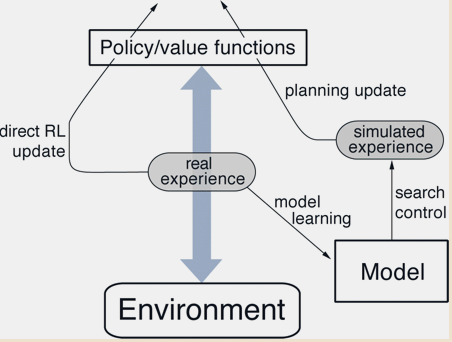
\includegraphics[width=.5\textwidth]{figures/dyna-architecture}
\end{center}
\caption{\
The general Dyna Architecture.\
Real experience, passing back and forth between the environment and the policy,\
affects policy and value functions in much the same way as does simulated experience generated by the model of the environment.\
}
\label{fig:dyna-architecture}
\end{figure}


\begin{table}
\beginalg
Initialize $Q(\curs,\cura)$ and $Model(\curs,\cura)$ for all $s\in\stateset$ and $\cura\in\actionset(S)$\\
\\
Loop:\\
\> $S \assign$ current (nonterminal) state\\
\> $A \assign$ \epsgreedy$(S,Q)$ \\
\> Take action $A$; observe reward $R$ and next state $S'$\\
\> Update Q-function: $Q(S,A) \assign (1-\alpha) Q(S,A) + \alpha \left( R + \df \max_{\cura\in\actionset(S)}Q(S',\cura)\right)$\\
\> $Model(S,A) \assign R, S'$ (assuming deterministic environment)\\
\> Loop repeat\\
\> Apply one-step tabular Q-learning to $S$, $A$, $R$, $S'$:\\
\> \> $S \assign$ random previously observed state\\
\> \> $A \assign$ random action previously taken in $S$\\
\> \> $R, S' \assign Model(S,A)$\\
\> \> Update Q-function: $Q(S,A) \assign (1-\alpha) Q(S,A) + \alpha \left( R + \df \max_{\cura\in\actionset(S)}Q(S',\cura) \right)$\\
Until a certain criterion is satisfied
\endalg
\caption{Tabular Dyna-Q}
\label{tab:alg:tabular-dyna-q}
\end{table}


\section{On-policy Prediction with Approximation}

XXX

\section{On-policy Control with Approximation}

XXX

\section{Off-policy Methods with Approximation}

XXX

\section{Eligibility Traces}



Eligibility traces are one of the basic mechanisms of reinforcement learning.
Almost any temporal-difference (TD) method,
such as Q-learning or Sarsa,
can be combined with eligibility traces to obtain a more general method that may learn more efficiently.

We have already seen one way of unifying TD and Monte Carlo methods:
the $n$-step TD methods \S\ref{sec:n-step}.
What eligibility traces offer beyond these is an elegant algorithmic mechanism
with significant computational advantages.

The mechanism is a short-term memory vector,
the \emph{eligibility trace} $\et{t} \in \reals^\wvectdim$
that parallels the long-term weight vector $\wvector{t} \in \reals^\wvectdim$.
The rough idea is that when a component of \wvector{t}\ participates in producing an estimated value,
then the corresponding component of \et{t}\ is bumped up and then begins to fade away.
Learning will then occur in that component of \wvector{t}\
if a nonzero TD error occurs before the trace falls back to zero.
The \emph{trace-decay parameter} $\tdparam\in[0,1]$
determines the rate at which the trace falls.

The primary computational advantage of eligibility traces over $n$-step methods
is that only a single trace vector is required
rather than a store of the last $n$ feature vectors.
Learning also occurs continually and uniformly in time
rather than being delayed and then catching up at the end of the episode.
In addition
learning can occur and affect behavior
immediately after a state is encountered rather than being delayed $n$ steps.


\subsection{The \tdparam-return}

In \S\ref{sec:n-step} we defined an $n$-step return
as the sum of the first $n$ rewards plus the estimated value of the state reached in $n$ steps,
each appropriately discounted.
The general form of that equation,
for any parameterized function approximator, is
\begin{equation}
\label{eq:nstep-return}
\nstepreturn{t}{t+n}
=
\reward{t+1} + \df \reward{t+2} + \df^2 \reward{t+3} + \cdots + \df^{n-1} \reward{t+n}
+ \df^n \valappr(\state{t+n}, \wvector{t+n-1})
\end{equation}

Now we note that a valid update can be done not just toward any $n$-step return,
but toward any average of $n$-step returns for different $n$s.
An example of such an average can be
the average of $3$-step return, $5$-step return, and $7$-step return,
\ie,
\begin{equation}
\frac{1}{3}(
\nstepreturn{t}{t+3}
+\nstepreturn{t}{t+5}
+\nstepreturn{t}{t+7}
)
\end{equation}

This is one example, but averaging produces a substantial new range of algorithms.
For example, we can average across many $n$-step returns
from $1$-step return to $\infty$-step return
to obtain another way of interrelating TD and Monte Carlo methods.
Nn principle, one could even average experience-based updates
with DP updates to get a simple combination of experience-based and model-based methods.

An update that averages simpler component updates is called a compound update.
The TD(\tdparam) algorithm can be understood as one particular way of averaging $n$-step updates.
This average contains all the $n$-step updates,
each weighted proportionally to $\tdparam^n$ (where $\tdparam\in[0,1]$),
and is normalized (to ensure that the weights sum to $1$).
The resulting update is toward a return, called the \tdparam-return , defined in its state-based form by

\begin{equation}
\label{eq:lambda-return}
\ldreturn{t} = (1-\tdparam) \sum_{n=1}^\infty \tdparam^{n-1} \nstepreturn{t}{t+n}
\end{equation}
where $(1-\tdparam) \sum_{n=1}^\infty \tdparam^{n-1} = 1$.
If the episode terminates at $t=T$,
then $\nstepreturn{t}{t+n} = \nstepreturn{t}{T} = \return{t}$ for all $n \geq T-t$,
thus,
\begin{equation}
\ldreturn{t} = (1-\tdparam) \sum_{n=1}^{T-t-1} \tdparam^{n-1} \nstepreturn{t}{t+n}
+ (1-\tdparam) \sum_{n=T-t}^\infty \tdparam^{n-1} \nstepreturn{t}{t+n}
= (1-\tdparam) \sum_{n=1}^{T-t-1} \tdparam^{n-1} \nstepreturn{t}{t+n}
+ \tdparam^{T-t-1} \return{t}.
\end{equation}

Note that if $\tdparam=1$, $\ldreturn{t}$ becomes the original return \return{t}.
Thus, updating value functions according to \tdparam-return is equivalent to Monte Carlo algorithm.
On the other hand, if $\tdparam=0$,
$\ldreturn{t}$ becomes $\nstepreturn{t}{t+1}$,
hence updating value functions according to \tdparam-return is equivalent to
the one-step temporal difference method,
\ie, TD($0$) method.

Now we define our first learning algorithm based on the \tdparam-return:
the \emph{off-line \tdparam-return algorithm}.
As an off-line algorithm,
it makes no changes to the weight vector during the episode.
Then, at the end of the episode,
a whole sequence of off-line updates are made according
to the semi-gradient method
using the \tdparam-return as the target.
The update rule of this method is
\begin{equation}
\label{eq:off-line-lambda-return-update}
\wvector{t+1} = \wvector{t}
+ \stepsize{t} \left( \ldreturn{t} - \valappr(\state{t}, \wvector{t})
\right) \nabla_{\wvector{}} \valappr(\state{t}, \wvector{t})
\end{equation}
for $t=0,\ldots, T-1$.
The \tdparam-return gives us
an alternative way of moving smoothly
between Monte Carlo and one-step TD methods
that can be compared with the $n$-step bootstrapping.

The above approach is what can be called the \emph{theoretical or forward} view of a learning algorithm.
For each state visited, we look forward in time to all the future rewards and decide how best to combine them.

\subsection{TD(\tdparam)}

TD(\tdparam) is one of the oldest and most widely used algorithms in reinforcement learning.
It was the first algorithm for which a formal relationship was shown between a more theoretical forward view
and a more computationally congenial backward view using eligibility traces.
Here we will show empirically that it approximates the off-line \tdparam-return algorithm
presented in the previous section.

TD(\tdparam) improves over the off-line \tdparam-return algorithm in three ways.
\begin{itemize}
\item It updates the weight vector on every step of an episode rather than only at the end,
thus its estimates is updated sooner (and may be better sooner).
\item Its computations are equally distributed in time
(rather than all at the end of the episode).
\item It can be applied to continuing problems rather than just to episodic problems.
\end{itemize}
The semi-gradient version of TD(\tdparam) with function approximation
will be shown below.

The \emph{eligibility trace} is a vector $\et{t} \in \reals^\wvectdim$
where the number of components of \et{t}\ is the same as that of \wvector{t}.
Whereas the \emph{weight vector}, \wvector{t}, is a long-term memory
accumulating over the lifetime of the system,
the eligibility trace is a short-term memory,
which typically lasts shorter than the length of an episode.
Eligibility traces assist in the learning process;
their only consequence is that they affect the weight vector,
and then the weight vector determines the estimated value.
At the same time, the eligibility traces plays a critical role
since that is what propagates future reward to the current one,
or equivalently, current reward back to the past states.

In TD(\tdparam),
the eligibility trace vector is initialized to zero at the beginning of the episode,
is incremented on each time step by the value gradient,
and then fades away by $\df \tdparam$
additively,
\ie,
\begin{eqnarray}
\nonumber
\et{t-1} &\assign& 0
\\
\et{t} &\assign& \df \tdparam \et{t-1} + \nabla_{\wvector{}} \valappr(\state{t}, \wvector{t}),
\ 0 \leq t \leq T
\label{eq:et:et-update}
\end{eqnarray}
where \df\ is the \emph{discount rate} and \tdparam\ is the \emph{trace-decay parameter}.

The eligibility trace keeps track of which components of the weight vector have contributed, positively or negatively,
to recent state valuations,
where ``recent'' is defined in terms of $\df \tdparam$.
The trace indicates the eligibility of each component of the weight vector for undergoing learning changes
should a reinforcing event occur where
the reinforcing events are the moment-by-moment one-step TD errors.
The TD error for state-value prediction is
\begin{equation}
\label{eq:et:td-error}
\tderror{t} \assign \reward{t+1} + \df \valappr(\state{t+1}, \wvector{t}) - \valappr(\state{t}, \wvector{t})
\end{equation}
Finally, the weight vector is updated on each step
proportionally to all three factors;
the step size,
the TD error,
and the eligibility trace,
\ie,
\begin{equation}
\label{eq:et:weight-vector-update}
\wvector{t+1} \assign \wvector{t} + \stepsize{t} \tderror{t} \et{t}.
\end{equation}

\tablename~\ref{tab:alg:et:semi-gradient} described the \emph{semi-gradient TD(\tdparam) algorithm} for estimating $\valappr \sim v_\pol$
using
(\ref{eq:et:et-update}),
(\ref{eq:et:td-error}),
and
(\ref{eq:et:weight-vector-update}).

\begin{table}
\beginalg
Inputs:\\
\> \pol\ to be evaluated
\\
\> differential function $\valappr: \nonterminalstateset \times \reals^\wvectdim \to \reals$
	such that $\valappr(\mathrm{terminal}, \cdot) = 0$
\\\\
Algorithm parameters:
\\
\> trace-decay parameter, $\tdparam \in [0,1]$, and step size, $\stepsize{t}>0$
\\\\
Initialize:
\\\\
\> Initialize value-function weights \wvector{}\ arbitrarily
\\\\
Loop for each episode:\\
\> Initialize \state\
\\
\> $\et{} \assign 0$
\\
\> Loop for each step of episode:
\\
\> \> Choose $\action{} \sim \pol(\cdot|\state{})$\\
\> \> Take action \action, observe \reward{}, $\state{}'$\\
%\> \> $\et{} \assign \df \tdparam \et{} + \nabla_{\wvector{}} \valappr(\state{}, \wvector{})$\\
\> \> $\tderror{} \assign \reward{} + \df \valappr(\state{}', \wvector{}) - \valappr(\state{}, \wvector{})$\\
\> \> $\wvector{} \assign \wvector{} + \stepsize{t} \tderror{} \et{}$\\
\> \> $\state{} \assign \state{}'$
\\
\> until $S'$ is terminal
\endalg
\caption{Semi-gradient TD(\tdparam) algorithm for estimating $\valappr \sim v_\pol$.}
\label{tab:alg:et:semi-gradient}
\end{table}


\subsection{Why TD(\tdparam) approximates the off-line \tdparam-return algorithm?}

Here we examine why TD(\tdparam) approximates the off-line \tdparam-return algorithm.

In this section, we drop the subscript $t$ from \wvector{t}.
Because of this, we can only prove thet TD(\tdparam) is \emph{approximately} the same as the off-line \tdparam-return algorithm.
In fact, they are different.

First, the $n$-step return at $t$ can be rewritten in terms of that at $t+1$ as follows.
\begin{eqnarray*}
\nstepreturn{t}{t+n}
&=& \reward{t+1} + \df \reward{t+2} + \df^2 \reward{t+3} + \cdots + \df^{n-1} \reward{t+n}
+ \df^n \valappr(\state{t+n}, \wvector{})
\\
&=& \reward{t+1} + \df \reward{t+2} + \df^2 \reward{t+3} + \cdots + \df^{n-1} \reward{t+n}
\\
&& + \df \valappr(\state{t+1}, \wvector{}) - \valappr(\state{t}, \wvector{})
\\
&& + \df(\df \valappr(\state{t+2}, \wvector{}) - \valappr(\state{t+1}, \wvector{}))
\\
&& + \cdots
\\
&& + \df^{n-1} (\df \valappr(\state{t+n}, \wvector{}) - \valappr(\state{t+n-1}, \wvector{}))
\\
&& + \valappr(\state{t}, \wvector{})
\\
&=& \reward{t+1} + \df \valappr(\state{t+1}, \wvector{}) - \valappr(\state{t}, \wvector{})
\\
&& + \df(\reward{t+2} + \df \valappr(\state{t+2}, \wvector{}) - \valappr(\state{t+1}, \wvector{}))
\\
&& + \cdots
\\
&& + \df^{n-1} (\reward{t+n} + \df \valappr(\state{t+n}, \wvector{}) - \valappr(\state{t+n-1}, \wvector{}))
\\
&& + \valappr(\state{t}, \wvector{}),
\end{eqnarray*}
thus, (\ref{eq:et:td-error}) implies
\begin{equation}
\label{eq:nusl}
\nstepreturn{t}{t+n}
= \tderror{t} + \df \tderror{t+1} +  \cdots + \df^{n-1} \tderror{t+n-1} + \valappr(\state{t}, \wvector{})
\end{equation}

\iffalse
\begin{eqnarray}
\nonumber
\nstepreturn{t}{t+n}
&=& \reward{t+1} + \df \reward{t+2} + \df^2 \reward{t+3} + \cdots + \df^{n-1} \reward{t+n}
+ \df^n \valappr(\state{t+n}, \wvector{})
\\
\nonumber
&=& \reward{t+1} + \df \reward{t+2} + \df^2 \reward{t+3} + \cdots + \df^{n-1} \reward{t+n}
+ \df^{n} \reward{t+n+1}
+ \df^{n+1} \valappr(\state{t+n+1}, \wvector{})
\\
\nonumber
&&
+ \df^n \valappr(\state{t+n}, \wvector{})
- \df^{n} \reward{t+n+1}
- \df^{n+1} \valappr(\state{t+n+1}, \wvector{})
\\
\nonumber
&=& \reward{t+1} + \df \left(\reward{t+2} + \df \reward{t+3} + \cdots + \df^{n-2} \reward{t+n}
+ \df^{n-1} \reward{t+n+1}
+ \df^{n} \valappr(\state{t+n+1}, \wvector{})
\right)
\\
\nonumber
&&
+ \df^n \valappr(\state{t+n}, \wvector{})
- \df^{n} \reward{t+n+1}
- \df^{n+1} \valappr(\state{t+n+1}, \wvector{})
\\
\nonumber
&=& \reward{t+1} + \df \nstepreturn{t+1}{t+n+1}
- \df^n \left( \reward{t+n+1} + \df \valappr(\state{t+n+1}, \wvector{}) - \valappr(\state{t+n}, \wvector{}) \right)
\\
&=& \reward{t+1} + \df \nstepreturn{t+1}{t+n+1} - \df^n \tderror{t+n}
\label{eq:difkc}
\end{eqnarray}
where
(\ref{eq:nstep-return}) and (\ref{eq:et:td-error}) are used.
\fi

Now (\ref{eq:nusl}) together with (\ref{eq:lambda-return}) implies that
\begin{eqnarray*}
\ldreturn{t} &=& (1-\tdparam) \sum_{n=1}^\infty \tdparam^{n-1} \nstepreturn{t}{t+n}
\\
&=& (1-\tdparam) \sum_{n=1}^\infty \tdparam^{n-1}
\left( \tderror{t} + \df \tderror{t+1} +  \cdots + \df^{n-1} \tderror{t+n-1} + \valappr(\state{t}, \wvector{}) \right)
\\
&=& (1-\tdparam) \sum_{n=1}^\infty \tdparam^{n-1}
\left(\sum_{k=0}^{n-1} \df^k \tderror{t+k} + \valappr(\state{t}, \wvector{}) \right)
\\
&=& (1-\tdparam) \sum_{n=1}^\infty \tdparam^{n-1}
\left(\sum_{k=0}^{n-1} \df^k \tderror{t+k} \right)
+ (1-\tdparam) \sum_{n=1}^\infty \tdparam^{n-1} \valappr(\state{t}, \wvector{})
\\
&=& (1-\tdparam) \sum_{n=1}^{\infty} \sum_{k=0}^{n-1} \tdparam^{n-1} \df^k \tderror{t+k}
+ (1-\tdparam) \sum_{n=1}^\infty \tdparam^{n-1} \valappr(\state{t}, \wvector{})
\\
&=& (1-\tdparam) \sum_{k=0}^{\infty} \sum_{n=k+1}^\infty \tdparam^{n-1} \df^k \tderror{t+k}
+ (1-\tdparam) \sum_{n=1}^\infty \tdparam^{n-1} \valappr(\state{t}, \wvector{})
\\
&=& (1-\tdparam) \sum_{k=0}^{\infty} \df^k \tderror{t+k} \sum_{n=k+1}^\infty \tdparam^{n-1}
+ \valappr(\state{t}, \wvector{})
\\
&=& \sum_{k=0}^{\infty} (\df \tdparam)^k \tderror{t+k} + \valappr(\state{t}, \wvector{})
\end{eqnarray*}
since $(1-\tdparam) \sum_{n=1}^\infty \tdparam^{n-1} = 1$,
thus
\begin{equation}
\ldreturn{t} - \valappr(\state{t}, \wvector{}) = \sum_{k=0}^{\infty} (\df \tdparam)^k \tderror{t+k}.
\end{equation}
If an episode ends at $t=T$, then $tderror{t}=0$ for $t\geq T$,
hence
\begin{equation}
\label{eq:bysig}
\ldreturn{t} - \valappr(\state{t}, \wvector{}) = \sum_{k=0}^{T-t-1} (\df \tdparam)^k \tderror{t+k}.
\end{equation}

Now we derived a formula for \et{t+n}\ using summation notation from the recursive formula (\ref{eq:et:et-update}).
\begin{eqnarray*}
\et{t+n} &=& \df \tdparam \et{t+n-1} + \nabla_{\wvector{}} \valappr(\state{t+n},\wvector{})
\\
&=& \df \tdparam \left(
\df \tdparam \et{t+n-2} + \nabla_{\wvector{}} \valappr(\state{t+n-1},\wvector{})
\right)
+ \nabla_{\wvector{}} \valappr(\state{t+n},\wvector{})
\\
&=& (\df \tdparam )^2 \et{t+n-2} + (\df \tdparam) \nabla_{\wvector{}} \valappr(\state{t+n-1},\wvector{})
+ \nabla_{\wvector{}} \valappr(\state{t+n},\wvector{})
\\
&\vdots&
\\
&=& (\df \tdparam )^{n} \nabla_{\wvector{}} \valappr(\state{t},\wvector{})
+ (\df \tdparam)^{n-1} \nabla_{\wvector{}} \valappr(\state{t+1},\wvector{})
%+ (\df \tdparam)^{n-2} \nabla_{\wvector{}} \valappr(\state{t+2},\wvector{})
+ \cdots
+ (\df \tdparam) \nabla_{\wvector{}} \valappr(\state{t+n-1},\wvector{})
+ \nabla_{\wvector{}} \valappr(\state{t+n},\wvector{}),
\end{eqnarray*}
thus,
\begin{equation}
\label{eq:vyduf}
\et{t+n} = \sum_{k=0}^n (\df \tdparam)^{n-k} \nabla_{\wvector{}} \valappr(\state{t+k},\wvector{}).
\end{equation}
(We can prove (\ref{eq:vyduf}) mathematically strictly using the mathematical induction.)

We also derive a formula for \wvector{t+n}\ using summation notation from the recursive formula (\ref{eq:et:weight-vector-update})
and (\ref{eq:et:td-error}).
\begin{eqnarray*}
\wvector{t+n} &=& \stepsize{} \tderror{t+n-1} \et{t+n-1} + \wvector{t+n-1}
\\
&=& \stepsize{} \left( \tderror{t+n-1} \et{t+n-1} + \tderror{t+n-2} \et{t+n-2} \right) + \wvector{t+n-2}
\\
&=& \stepsize{} \left(
\tderror{t+n-1} \et{t+n-1} + \tderror{t+n-2} \et{t+n-2} + \cdots + \tderror{t+1} \et{t+1} + \tderror{t} \et{t}
\right)
+ \wvector{t}
\end{eqnarray*}
where we drop the subscript from the step size \stepsize{t}.
Thus,
\begin{equation}
\label{eq:nuasdk}
\wvector{t+n} = \stepsize{} \sum_{j=0}^{n-1}  \tderror{t+j} \et{t+j} + \wvector{t}.
\end{equation}

Now combining (\ref{eq:vyduf}) and (\ref{eq:nuasdk}) yields
\begin{eqnarray}
\nonumber
\wvector{t+n} - \wvector{t}
&=& \stepsize{} \sum_{j=0}^{n-1}  \tderror{t+j} \et{t+j}
\\
\nonumber
&=& \stepsize{} \sum_{j=0}^{n-1}  \tderror{t+j} 
\sum_{k=0}^j (\df \tdparam)^{j-k} \nabla_{\wvector{}} \valappr(\state{t+k},\wvector{}).
\\
\nonumber
&=& \stepsize{} \sum_{j=0}^{n-1} \sum_{k=0}^j (\df \tdparam)^{j-k}
\tderror{t+j} \nabla_{\wvector{}} \valappr(\state{t+k},\wvector{}).
\\
\nonumber
&=& \stepsize{} \sum_{k=0}^{n-1} \sum_{j=k}^{n-1} (\df \tdparam)^{j-k}
\tderror{t+j} \nabla_{\wvector{}} \valappr(\state{t+k},\wvector{})
\\
\nonumber
&=& \stepsize{} \sum_{k=0}^{n-1} \nabla_{\wvector{}} \valappr(\state{t+k},\wvector{})
\sum_{j=k}^{n-1} (\df \tdparam)^{j-k} \tderror{t+j}
\\
\nonumber
&=& \stepsize{} \sum_{k=0}^{n-1} \nabla_{\wvector{}} \valappr(\state{t+k},\wvector{})
\sum_{j=0}^{n-k-1} (\df \tdparam)^{j} \tderror{t+k+j}
\\
\label{eq:bgusdf}
&=& \stepsize{} \sum_{k=0}^{n-1} \nabla_{\wvector{}} \valappr(\state{t+k},\wvector{})
\sum_{j=0}^{n+t-(t+k)-1} (\df \tdparam)^{j} \tderror{(t+k)+j}.
\end{eqnarray}
Now if we substitute $T-t$ for $n$ in (\ref{eq:bgusdf}),
(\ref{eq:bysig}) implies
\begin{eqnarray}
\nonumber
\wvector{T} - \wvector{t}
&=& \stepsize{} \sum_{k=0}^{T-t-1} \nabla_{\wvector{}} \valappr(\state{t+k},\wvector{})
\sum_{j=0}^{T-(t+k)-1} (\df \tdparam)^{j} \tderror{(t+k)+j}
\\
\nonumber
&=& \stepsize{} \sum_{k=0}^{T-t-1} \nabla_{\wvector{}} \valappr(\state{t+k},\wvector{})
\left( \ldreturn{t+k} - \valappr(\state{t+k}, \wvector{}) \right)
\\
\nonumber
&=& \stepsize{} \sum_{k=0}^{T-t-1}
\left( \ldreturn{t+k} - \valappr(\state{t+k}, \wvector{}) \right)
\nabla_{\wvector{}} \valappr(\state{t+k},\wvector{}).
\\
&=& \stepsize{} \sum_{k=t}^{T-1}
\left( \ldreturn{k} - \valappr(\state{k}, \wvector{}) \right)
\nabla_{\wvector{}} \valappr(\state{k},\wvector{}).
\label{eq:ishfg}
\end{eqnarray}

Now observer that the semi-gradient update rule for off-line \tdparam-return algorithm
(\ref{eq:off-line-lambda-return-update}) implies that
\begin{eqnarray}
\nonumber
\wvector{T}
&=& \stepsize{} \left( \ldreturn{T-1} - \valappr(\state{T-1}, \wvector{}) \right) \nabla_{\wvector{}} \valappr(\state{T-1}, \wvector{})
+ \wvector{T-1}
\\
\nonumber
&=&
\stepsize{} \left( \ldreturn{T-1} - \valappr(\state{T-1}, \wvector{}) \right) \nabla_{\wvector{}} \valappr(\state{T-1}, \wvector{})
+ \stepsize{} \left( \ldreturn{T-2} - \valappr(\state{T-2}, \wvector{}) \right) \nabla_{\wvector{}} \valappr(\state{T-2}, \wvector{})
+ \wvector{T-2}
\\
\nonumber
&\vdots&
\\
\nonumber
&=&
\stepsize{} \left( \ldreturn{T-1} - \valappr(\state{T-1}, \wvector{}) \right) \nabla_{\wvector{}} \valappr(\state{T-1}, \wvector{})
+ \cdots
+ \stepsize{} \left( \ldreturn{t} - \valappr(\state{t}, \wvector{}) \right) \nabla_{\wvector{}} \valappr(\state{t}, \wvector{})
+ \wvector{t}
\\
&=& \stepsize{} \sum_{k=t}^{T-1}
\left( \ldreturn{k} - \valappr(\state{k}, \wvector{}) \right)
\nabla_{\wvector{}} \valappr(\state{k},\wvector{})
+ \wvector{t}
\label{eq:gudif}
\end{eqnarray}
assuming that $\stepsize{t} = \stepsize{}$ and $\wvector{t}=\wvector{}$ for all $t$.
(We can prove (\ref{eq:gudif}) in a mathematically strict way using the mathematical induction.)
Comparing (\ref{eq:ishfg}) with (\ref{eq:gudif}) implies that
the off-line \tdparam-return algorithm and TD(\tdparam) are equivalent
when we drop $t$ from \wvector{t} and \stepsize{t}.
Therefore we have shown that TD(\tdparam) approximates the off-line \tdparam-return algorithm.


\subsection{Tabular TD(\tdparam)}

In the previous sections, we describe TD(\tdparam) for function approximation cases.
Since the tabular case is a special case of the function approximation,
we can readily derived TD(\tdparam) algorithm for the tabular case.

Suppose that the set of all the states, \stateset, is finite
and there is a one-to-one mapping $\indexstatemapping: \{1,\ldots, \numstates\} \to \stateset$
which maps an (integer) index to a state.
Let $\wvector{} \in \reals^{\numstates}$
be the weight vector such that
$\wvector{i} = V(\indexstatemapping(i))$,
\ie, \wvector{i}\ represents the state value function for the $i$th state
(where the order is defined by \indexstatemapping).
Then we have
\begin{equation}
\label{eq:appr-val-fcn-tabular-case}
\valappr(\state{}, \wvector{}) = w_{\indexstatemapping^{-1}(\state{})}.
\end{equation}

Now we apply (\ref{eq:appr-val-fcn-tabular-case}) to each of the three update rule for TD(\tdparam);
(\ref{eq:et:et-update}),
(\ref{eq:et:td-error}),
and
(\ref{eq:et:weight-vector-update}).
We first derived the gradient of $\valappr(\state{}, \wvector{})$ with respect to \wvector{}
for each $\state{} \in \stateset$.
Note that
\begin{equation}
\frac{\partial}{\partial \wvector{i}} \valappr(\state{}, \wvector{})
= \delta_{\indexstatemapping^{-1}(\state{}), i}
= \left\{\begin{array}{ll}
	1 & \mbox{if } \indexstatemapping(i)= \state{}
	\\
	0 & \mbox{otherwise}
\end{array}\right.
\end{equation}
where $\delta_{\cdot, \cdot}$ is the Kronecker delta function
defined by
\begin{equation}
\delta_{i,j}
= \left\{\begin{array}{ll}
	1 & \mbox{if } i=j,
	\\
	0 & \mbox{otherwise.}
\end{array}\right.
\end{equation}
Therefore the gradient is
\begin{equation}
\label{eq:viskgjh}
\nabla_\wvector{} \valappr(\state{}, \wvector{}) = e_{\indexstatemapping^{-1}(\state{})}
\end{equation}
where $e_i\in\reals^\numstates$ is the $i$th unit vector 
whose entries are all zero except the $i$th entry which is $1$.


Now let us apply (\ref{eq:viskgjh}) to (\ref{eq:et:et-update}), (\ref{eq:et:td-error}),
and (\ref{eq:et:weight-vector-update}).
First, the eligibility trace update (\ref{eq:et:et-update}) becomes
\begin{eqnarray}
\nonumber
\et{} \assign 0 \in \reals^\numstates
\\
\et{t} &\assign& \df \tdparam \et{t-1} + \nabla_{\wvector{}} \valappr(\state{t}, \wvector{t}),
\ 0 \leq t \leq T
\end{eqnarray}












\section{Appendix: conditional probability and expected value}
\label{sec:rl-app}


Suppose that we have a sequence of random variables, $X$, $Y$, and $Z$
with supports \suppx, \suppy, and \suppz.

Note that the definition of the conditional probability implies that
for all $x\in\suppx$, $y\in\suppy$, $z\in\suppz$ such that $p_Y(y)\neq0$ and $p_Z(z)\neq 0$,
\begin{equation}
\label{eq:vusg-1}
p_{X|Y}(x|y)
= \frac{p_{X,Y}(x,y)}{p_Y(y)}
\Leftrightarrow
p_{X,Y}(x,y) = p_{X|Y}(x|y) p_Y(y).
\end{equation}


\begin{equation}
\label{eq:vusg-2}
p(x,y|z)
= \frac{p(x,y,z)}{p(z)}
= \frac{p(x,y,z)}{p(y,z)} \frac{p(y,z)}{p(z)}
= p(x|y,z) p(y|z).
\end{equation}

Then (\ref{eq:vusg-1}) implies
\begin{eqnarray*}
\lefteqn{
\Expect(X)
= \int_\suppx x p_X(x) dx
}
\\
&=& \int_\suppx x \left(\int_\suppy p_{X,Y}(x,y) dy \right) dx
= \int_\suppx x \left(\int_\suppy p_{X|Y}(x|y)p_Y(y) dy \right) dx
\\
&=& \int_\suppy \int_\suppx x p_{X|Y}(x|y)p_Y(y) dx dy
= \int_\suppy \left( \int_\suppx x p_{X|Y}(x|y) dx \right) p_Y(y) dy
\\
&=& \int_\suppy \Expect (X|Y=y) p_Y(y) dy
= \Expect_Y \Expect_{X|Y} (X|Y),
\end{eqnarray*}
\begin{equation}
\Expect(X) = \Expect_{X|Y} (X|Y),
\end{equation}
and (\ref{eq:vusg-2}) implies
\begin{eqnarray*}
\lefteqn{
\Expect(X|Z=z)
= \int_\suppx x p_{X|Z}(x|z) dx
}
\\
&=& \int_\suppx x \left(\int_{\suppy} p_{X,Y|Z}(x,y|z) dy \right) dx
= \int_\suppx x \left(\int_{\suppy} p_{X|Y,Z}(x|y,z) p_{Y|Z}(y|z) dy \right) dx
\\
&=& \int_\suppy \int_\suppx x p_{X|Y,Z}(x|y,z) p_{Y|Z}(y|z) dx dy
= \int_\suppy \left( \int_\suppx x p_{X|Y,Z}(x|y,z) dx \right) p_{Y|Z}(y|z) dy
\\
&=& \int_\suppy \Expect(X|Y=y,Z=z) p_{Y|Z}(y|z) dy
= \Expect_{Y|Z=z} \Expect(X|Y,Z=z),
\end{eqnarray*}
\ie,
\begin{equation}
\label{eq:dkci}
\Expect(X|Z=z)
= \Expect_{Y|Z=z} \Expect(X|Y,Z=z).
\end{equation}
